\documentclass{article}
\usepackage{tikz}
\usepackage{mathtools}

\newcommand\then{\rightarrow}
\newcommand\liff{\leftrightarrow}
\newcommand\lxor{\oplus}
\author{Sandra Kohl, Jan Hendrik Kirchner, Max Bernhard Ilsen}

\begin{document}
\section{Exercise \textit{(Multi-Layer Perceptron (8p))}}
\begin{enumerate}
    \item Draw multi-layer perceptron to solve each given logical function
        below.\\
        \scriptsize
        (We assume a threshold $\Theta = 1$ for each neuron.
        That is, neurons fire if they have an activation of 1 or higher, and
        they do not fire if they have an activation lower than 1.)
        \normalsize
        \begin{enumerate}
            \item $x1 \lxor x2$\\
                \begin{center}
                    \begin{minipage}{8cm}
                        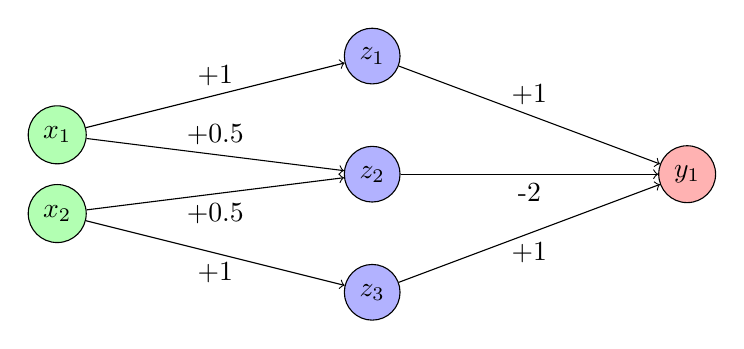
\begin{tikzpicture}
                            \path
                            (0,3) node[circle,draw,fill=green!30](x1) {$x_1$}
                            (0,2) node[circle,draw,fill=green!30](x2) {$x_2$}
                            (4,4) node[circle,draw,fill=blue!30](z1) {$z_1$}
                            (4,2.5) node[circle,draw,fill=blue!30](z2) {$z_2$}
                            (4,1) node[circle,draw,fill=blue!30](z3) {$z_3$}
                            (8,2.5) node[circle,draw,fill=red!30](y1) {$y_1$};

                            \draw[->] (x1) -- node[align=center,above]{+1} (z1);
                            \draw[->] (x1) -- node[align=center,above]{+0.5} (z2);
                            \draw[->] (x2) -- node[align=center,below]{+0.5} (z2);
                            \draw[->] (x2) -- node[align=center,below]{+1} (z3);

                            \draw[->] (z1) -- node[align=center,above]{+1} (y1);
                            \draw[->] (z2) -- node[align=center,below]{-2} (y1);
                            \draw[->] (z3) -- node[align=center,below]{+1} (y1);
                        \end{tikzpicture}
                    \end{minipage}
                \end{center}
            \item $(x_1 \land x_4) \lor (x_2 \land x_3)$\\
                \begin{center}
                    \begin{minipage}{8cm}
                        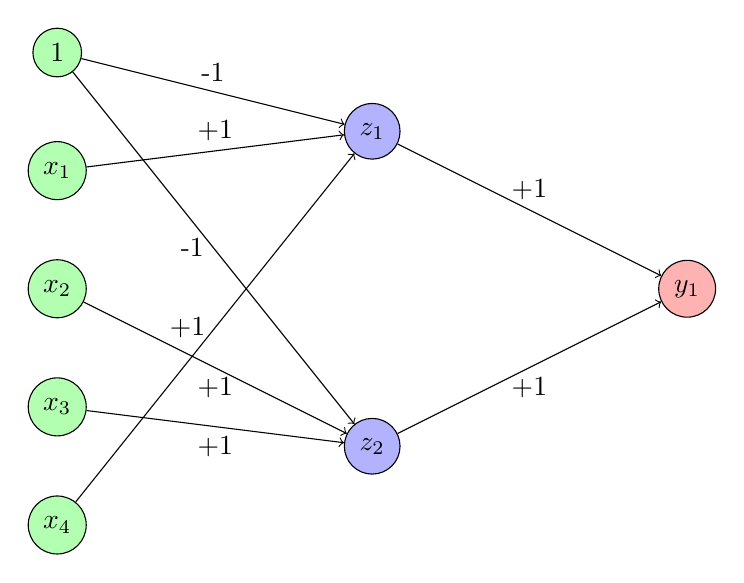
\begin{tikzpicture}
                            \path
                            (0,6) node[circle,draw,fill=green!30](x0) {$1$}
                            (0,4.5) node[circle,draw,fill=green!30](x1) {$x_1$}
                            (0,3) node[circle,draw,fill=green!30](x2) {$x_2$}
                            (0,1.5) node[circle,draw,fill=green!30](x3) {$x_3$}
                            (0,0) node[circle,draw,fill=green!30](x4) {$x_4$}
                            (4,5) node[circle,draw,fill=blue!30](z1) {$z_1$}
                            (4,1) node[circle,draw,fill=blue!30](z2) {$z_2$}
                            (8,3) node[circle,draw,fill=red!30](y1) {$y_1$};

                            \draw[->] (x0) -- node[align=center,above] {-1} (z1);
                            \draw[->] (x0) -- node[align=center,below,left] {-1} (z2);
                            \draw[->] (x1) -- node[align=center,above] {+1} (z1);
                            \draw[->] (x4) -- node[align=center,above,left] {+1} (z1);
                            \draw[->] (x2) -- node[align=center,below] {+1} (z2);
                            \draw[->] (x3) -- node[align=center,below] {+1} (z2);
                            \draw[->] (z1) -- node[align=center,above] {+1} (y1);
                            \draw[->] (z2) -- node[align=center,below] {+1} (y1);
                        \end{tikzpicture}
                    \end{minipage}
                \end{center}
            \item $x_1 \lor (x_2 \land x_3)$\\
                \begin{center}
                    \begin{minipage}{8cm}
                        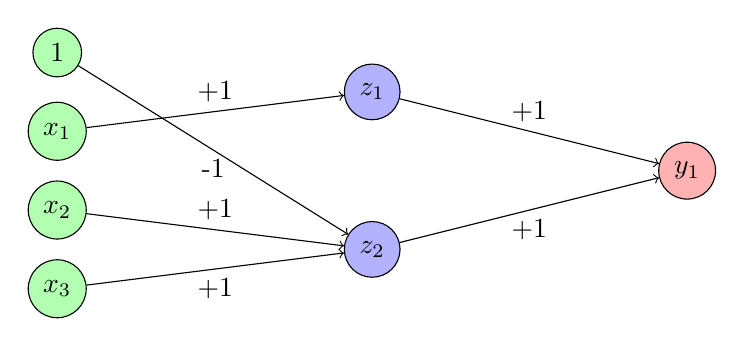
\begin{tikzpicture}
                            \path
                            (0,3) node[circle,draw,fill=green!30](x0) {$1$}
                            (0,2) node[circle,draw,fill=green!30](x1) {$x_1$}
                            (0,1) node[circle,draw,fill=green!30](x2) {$x_2$}
                            (0,0) node[circle,draw,fill=green!30](x3) {$x_3$}
                            (4,2.5) node[circle,draw,fill=blue!30](z1) {$z_1$}
                            (4,0.5) node[circle,draw,fill=blue!30](z2) {$z_2$}
                            (8,1.5) node[circle,draw,fill=red!30](y1) {$y_1$};

                            \draw[->] (x0) -- node[below] {-1} (z2);
                            \draw[->] (x1) -- node[above] {+1} (z1);
                            \draw[->] (x2) -- node[above] {+1} (z2);
                            \draw[->] (x3) -- node[below] {+1} (z2);
                            \draw[->] (z1) -- node[above] {+1} (y1);
                            \draw[->] (z2) -- node[below] {+1} (y1);
                        \end{tikzpicture}
                    \end{minipage}
                \end{center}
        \end{enumerate}
        \newpage
    \item Calculate the following derivatives:
        \begin{enumerate}
            \item
                \begin{align*}
                    f(x) &= \frac{1}{1+exp(-\lambda x)}  = (1+exp(-\lambda
                    x))^{-1}\\
                    f'(x) &= (-1)*(1+exp(-\lambda x))^{-2}*exp(-\lambda
                    x)*(-\lambda)\\
                    &= \frac{\lambda}{1+exp(-\lambda x)}*\frac{exp(-\lambda
                x)}{1+exp(-\lambda x)}\\
                &= \frac{\lambda}{1+exp(-\lambda x)}*\frac{1+exp(-\lambda
            x)-1}{1+exp(-\lambda x)}\\
            &= \frac{\lambda}{1+exp(-\lambda x)}*(1-\frac{ 1}{1+exp(-\lambda
        x)})\\
        &= \lambda*f(x)*(1-f(x))
    \end{align*}
\item
    \begin{align*}
        f(x) &= \frac{2}{1+exp(-x)} -1  = 2*(1+exp(-x))^{-1}\\
        f'(x) &= (-2)*(1+exp(- x))^{-2}*exp(-x)*(-1)\\
              &= 2*(1+exp(- x))^{-2}*exp(-x) \\
              &= \frac{2}{1+exp(-x)}*\frac{exp(-x)}{1+exp(- x)}\\
              &= \frac{2}{1+exp(-x)}*\frac{1+exp(-x)-1}{1+exp(- x)}\\
              &= \frac{2}{1+exp(-x)}*(1-\frac{1}{1+exp(- x)})\\
              &= \frac{1}{2}(\frac{2}{1+exp(-x)})*(2-\frac{2}{1+exp(-x)})\\
              &= \frac{1}{2}(1+\frac{2}{1+exp(-x)} -1)*(1-\frac{2}{1+exp(-x)}+1)\\
              &= \frac{1}{2}(1+f(x))*(1-f(x))
    \end{align*}
        \end{enumerate}
    \item Write down a general sigmoid function and its derivative.
        \begin{align*}
            f(x) &= \frac{|b-a|}{1+exp(-x)}+a  =
            |b-a|*(1+exp(-x))^{-1}+a\\
            f'(x) &= -|b-a|*(1+exp(- x))^{-2}*exp(-x)*(-1)\\
                  &= \frac{|b-a|}{1+exp(- x)}*\frac{exp(-x)}{1+exp(- x)}\\
                  &= \frac{|b-a|}{1+exp(- x)}*\frac{1+exp(-x)-1}{1+exp(- x)}\\
                  &= \frac{|b-a|}{1+exp(-x)}*(1-\frac{1}{1+exp(- x)})\\
                  &= \frac{1}{|b-a|}(\frac{|b-a|}{1+exp(-x)})*(|b-a|-\frac{|b-a|}{1+exp(-x)})\\
                  &= \frac{1}{|b-a|}(a+\frac{|b-a|}{1+exp(-x)}
            -a)*(b-\frac{|b-a|}{1+exp(-x)}-a) \text{ for } b \geq a\\
            &= \frac{1}{|b-a|}(-a+f(x))*(b-f(x))\\
        \end{align*}
\end{enumerate}

\section{Exercise \textit{(Backpropagation (4p))}}
\begin{enumerate}
    \item How to avoid local minima in backpropagation?\\
        \\
        If we repeat the training procedure several times, we will have gotten
        multiple different minima. Depending on the amount of times we have
        repeated it, the minimum of the local minima is then likely to
        be the global minimum as well.\\
        Another method to avoid local minima is simulated annealing: We add
        random noise to the weights to be able to "hop" out of local minima.
        Reducing the noise over time will help to not pass over the actual
        global minimum.
    \item Explain the generalization and avoiding overfitting.\\
        \\
        Generalization is basically a measure for the goodness of the fit of our
        weights to the test data: How well do our weights perform for another
        data set with the same underlying distribution?\\After several updates
        during the training procedure, our weights will adapt very strongly to
        the training examples, and it may come to overfitting: Instead of
        accounting for noise in the training data and giving a general result,
        our weights can only explain the training data but not any given test
        data. Hence, the error for our training data set will steadily decrease
        while the error for the test data set may increase again after a certain
        amount of weight updates.\\
        Overfitting can be avoided using weight decay. If we stop the weights
        from growing indefinitely, they can no longer reach numbers that are
        highly spezialized to the examples in our training data set without
        giving good results for a test data set as well.
    \item To prevent overly large weights which cause the high sensitivity of inputs, we apply the
        quadratic regularization term in the error function. Use gradient descent to minimize this
        error function.\\
        \\
        (See slide 48 of "ML-7 Neural Networks" for gradient descent on first
        summand.)
        \begin{align*}
            E[\{w\}] &= \frac{1}{2}\sum_{i=1..|D|}(t^i-y(x^i))^2+\frac{\beta}{2}
            \sum_{w \in \{w\}}w^2\\
            \Delta w_{jk}(x) &= -\epsilon \frac{\delta E}{\delta w_{jk}(m,n)}\\
                             &= -\epsilon * -\sum_{i=1..|D|}(t^i-y(x^i))^2
            \frac{\delta}{\delta w_{jk}(m,n)}y(x^i) + \sum_{w \in \{w\}}\beta w
        \end{align*}

\end{enumerate}
\end{document}
